\chapter{The Ordinal Serial Encoding Model}
The Ordinal Serial Encoding (OSE) model \parencite{Choo2010} is an NEF and SPA based model of serial recall.
It was able to reproduce various effects found in human recall data such as the primacy effect, recency effect, and transposition gradients in serial and delayed forward recall.
Within the context-unified encoding (CUE) memory model it provides the basis for the short-term memory component.

In the OSE, $m$ presented items $\vc v_i$ are bound to fixed position vectors $\vc p_i$ and stored in two memory traces
\begin{align}
    \osestm &= \sum_{i=1}^m \osestmdecay^{m - i} \bind(\vc v_i, \vc p_i) \\
    \oseepis &= \sum_{i=1}^m \oseepisscale^{m - i} \bind(\vc v_i, \vc p_i)
\end{align}
with decay factor $\osestmdecay < 1$ and scaling factor $\oseepisscale > 1$.
The memory traces $\osestm$ and $\oseepis$ represent the short-term and episodic memory store, respectively.
The binding operation $\bind$ used here is circular convolution, but it could be worth exploring the effect of other binding operations in the future.
The recall of an item is given by unbinding the corresponding position vector as
\begin{equation}
    \vc v_i \approx \bind^+\big(\osestm + \oseepis, \vc p_i\big) \text{.}
\end{equation}
These encoding equations produce the primacy and recency effect due to the differential effect of the decay and scaling factors $\osestmdecay$ and $\oseepisscale$.

For the neural implementation, each memory trace can be stored in an integrator with some additional processes for updating and unbinding the recalled item.
For the integration within the CUE memory model, the episodic memory trace is replaced by a version based on the temporal context model presented in the next chapter.
This introduces a more plausible episodic memory, storing experiences in actual synaptic weight changes rather than in the activities of a neural population.
In addition, the recall process needs to be adjusted to integrate information from the exchanged episodic memory component (\cref{sec:recall}).


\section{Neural STM implementation}
In the CUE model, the short-term memory buffer of the OSE model is implemented as depicted in \cref{fig:ose-flip-flop}.
The network gets an item and position Semantic Pointer as input which are bound together.
The bound result is added into the memory trace stored in \pop{combined} as long as it does not receive the \nin{input\_store} signal.
Once the \nin{input\_store} signal is received, the contents from \pop{combined} are transferred to the $\osestm$ populations.
Items are decoded from the memory via the approximate inverse circular convolution.
The decay factor of $\osestmdecay = 0.9775$ is taken from the original OSE implementation \parencite{Choo2010} and is implemented on the connection from $\osestm$ to \pop{combined}.
\begin{figure}
    \centering
    \begin{tikzpicture}[nef]
        \graph [no placement] {
            item/"item $\vc v$" [x=-0.5, y=0, ext];
            pos/"position $\vc p$" [x=-0.5, y=-1, ext];
            bind/"$\circledast$" [x=2, y=-0.5, net];
            diff1/"" [x=4, y=-0.5, ea];
            combined/"" [x=7, y=-0.5, ea];
            combinedlbl/"{\lato combined}" [x=7, y=0.1];
            diff2/"" [x=7, y=-3, ea];
            mem/"$\osestm$" [x=4, y=-3, ea];
            recall/"$\circledast^{-1}$" [x=2, y=-3, net];
            out/"recalled $\hat{\vc{v}}$" [x=-0.5, y=-3, ext];
            store/"input\_store" [x=-0.5, y=-2, ext];
            invstore/"" [x=6, y=-1.5, pnode];

            item -> [out=0, in=170] bind;
            pos -> [out=0, in=190] bind;
            bind -> diff1 -> combined -> diff2 -> mem -> ["\osestmdecay" {auto, yshift=3mm, xshift=1mm}] diff1;
            combined -> [bend right, "$-1$"] diff1;
            mem -> [bend right, "$-1$" below] diff2;
            mem -> recall;
            pos -> [out=0, in=90] recall;
            recall -> out;

            store -> [out=0, in=225, inhibit] diff1;
            store -> [out=0, in=200, "$-1$" {below, very near end}] invstore -> [inhibit] diff2;
            bias/"$1$" [x=5, y=-1.25, ext] -> invstore;
        };
    \end{tikzpicture}
    \caption[Implementation of the OSE short-term memory trace $\osestm$ with the NEF.]{Implementation of the OSE short-term memory trace $\osestm$ with the NEF\@. See text for additional details.}\label{fig:ose-flip-flop}
\end{figure}


\section{Neural position counting}\label{sec:posnet}
For the OSE it is necessary to keep track of the ordinal position of the current item.
The CUE model extends the OSE to do this also in neurons.
\Cref{fig:posnet} shows the network implementing this functionality.
All ensembles in this network are implementing a threshold at zero so that represented values are always positive.
The \pop{state} ensemble array has one ensemble for each possible position and only the ensemble for the current position is active.
This is ensured by providing a small negative bias ($-0.2$) to all ensembles to prevent spontaneous activity.
Furthermore, a recurrent connection with $\syntau = \SI{0.1}{\second}$ decoding a constant of $1.2$ keeps the current position in a state of stable activity.
\begin{figure} 
    \centering
    \begin{tikzpicture}[nef]
        \graph [no placement] {
            inputinc/"increment" [x=-2, y=0, ext] -> ["\small $\syntau = \SI{5}{\milli\second}$" below]
            red/"" [x=2, y=0, rect] ->
            reg/"" [x=4, y=0, rect];

            inputinc -> [bend left, "\small $-1,\ \syntau = \SI{50}{\milli\second}$"] red;
            adv/"" [x=6, y=-1, ea, inner sep=0.25ex];
            advrect/"" [x=6, y=-1, rect];
            advlbl/"{\lato advance threshold}" [anchor=west, x=6.4, y=-1];

            state/"" [x=3.5, y=-3, ea, inner sep=0.25ex];
            staterect/"" [x=3.5, y=-3, rect];
            statelbl/"{\lato state}" [x=2.9, y=-3.3];

            inhibit/"" [x=6, y=-5, ea, inner sep=0.25ex];
            inhibitrect/"" [x=6, y=-5, rect];
            inhibitlbl/"{\lato inhibit threshold}" [anchor=west, x=6.4, y=-5];

            reg -> ["\small $0.8 \Heavi(x) \imat$" auto] adv;
            adv -> [bend left, "\small $\mat T_2,\ \syntau = \SI{0.1}{\second}$" {below, align=left, very near start, xshift=1.3cm}] state;
            state -> [bend left, "\small $\mat T_1$" above] adv;
            state -> output [x=7, y=-3, ext];
            state -> [bend left] inhibit;
            inhibit -> [bend left, "\small $\mat T_3 \Heavi(\vc x)$" {below, xshift=-5mm, near end}] state;
            bias1/"$-0.6$" [x=3.5, y=-5, ext] -> inhibit;
            bias2/"$-0.2$" [x=2, y=-3, ext] -> state;
            state -> [out=90, in=160, distance=2cm, "\small $1.2 \Heavi(\vc x)$" above] state;

            gating/"gate signal" [x=4, y=1, ext] -> reg;
        };
    \end{tikzpicture}
    \caption[Implementation of position counting with the NEF\@.]{Implementation of position counting with the NEF\@. See text for details.}\label{fig:posnet}
\end{figure}

To advance to the next position a signal with a rising edge has to be provided to the \nin{increment} input.
To detect the rising edge, a differentiator ensemble is used that receives its input via two connections where one connection has a fast synaptic time constant ($\syntau = \SI{5}{\milli\second}$) and the other connection has a slow synaptic time constant ($\syntau = \SI{50}{\milli\second}$) and a transform of $-1$ (\cref{sec:differentiator}).
The output is fed through a gate ensemble that can be inhibited to prevent position increments.

Then the Heaviside step function is decoded from the \pop{gate signal} and fed into the \pop{advance threshold} ensemble array scaled by a factor of \num{0.8}.
The output of \pop{state} is also fed into \pop{advance threshold} with the transform
\begin{equation}
    \mat T_1 = \sbr{\begin{array}{cccc}
        0 & -1 & -1 & \cdots \\
        -1 & 0 & -1 & \cdots \\
        -1 & -1 & 0 & \cdots \\
        \vdots & \vdots & \vdots & \ddots
    \end{array}}
\end{equation}
which inhibits all ensembles except the one corresponding to the current position.
This ensemble only becomes active when a rising edge for the \pop{increment} input is detected.
The \pop{advance threshold} ensemble projects back to the \pop{state} ensembles with a transform of
\begin{equation}
    \mat T_2 = \sbr{\begin{array}{ccccc}
        0 & 0 & \cdots & 0 & 0 \\
        2 & 0 & \cdots & 0 & 0 \\
        0 & 2 & \cdots & 0 & 0 \\
        \vdots & \vdots & \ddots & \vdots & \vdots \\
        0 & 0 & \cdots & 2 & 0
    \end{array}}
\end{equation}
to excite the population representing the next position.

When the next position gets active, the old position needs to be inhibited at some point to prevent two positions from being active at the same time.
This is done via the \pop{inhibit threshold} ensemble array.
It receives a bias input of \num{-0.6} and input from the decoded constant from \pop{state}.
Once the threshold (decoded as Heaviside step function) is exceeded, the previous and next item are inhibited with the transform given by
\begin{equation}
    \mat T_3 = -\sbr{\begin{array}{ccccc}
            0 & 2 & 0 & \cdots & 0 \\
            0 & 0 & 2 & \cdots & 0 \\
            \vdots & \vdots & \vdots & \ddots & \vdots \\
            0 & 0 & 0 & \cdots & 2 \\
            2 & 0 & 0 & \cdots & 0
    \end{array}} - \sbr{\begin{array}{ccccc}
        0 & 0 & \cdots & 2 & 0 \\
        0 & 0 & \cdots & 0 & 2 \\
        2 & 0 & \cdots & 0 & 0 \\
        0 & 2 & \cdots & 0 & 0 \\
        \vdots & \vdots & \ddots & \vdots & \vdots
    \end{array}} \text{.}
\end{equation}
An example of how these component interact to advance the represented position is given in \cref{fig:pos-example}.
\begin{figure}
    \centering
    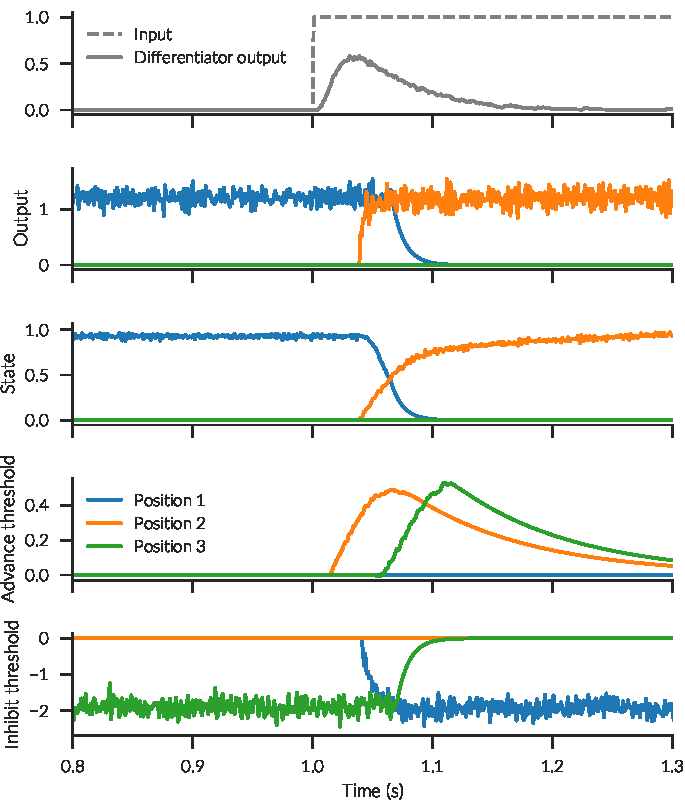
\includegraphics{figures/pos-example}
    \caption[Position increment in the position counting network.]{Position increment in the position counting network. The top-most plot shows the input signal and output of the differentiator. The following plots from top to bottom show: Heaviside output of the network, representation in the \pop{state} ensembles, transformed input to the \pop{state} ensembles from the \pop{advance threshold} ensembles, and transformed input from the \pop{inhibit threshold} ensembles.}\label{fig:pos-example}
\end{figure}
